\section{\sysname}
\label{sec:design}
Our design for \sysname focus on avoiding costly, unnecessary invocations of the network stack.
Envoy prides itself on being application agnostic, which leads to the helpful ability to auto-inject Envoy into microservices.
However, this abstract requires unnecessary invocations of the network stack.
In Figure-\ref{fig:no_kmap} we highlight in red all the calls to the network stack for the path of a single request.
Then, in Figure-\ref{fig:kmap} we show the reduction in those calls by using Kmap instead of the network stack for local data transfer.

\sysname works by using LD\_PRELOAD to load augmented network calls before libc regular calls.
Then, when Envoy and the microservice invoke read or write calls locally, rather than passing the data
into the network stack, we use \sysname's shared buffers to efficiently transfer the data.
Thus, we must load the shared library for both the Envoy sidecar and the microservices.
The two critical challenges to realizing \sysname are:
\begin{enumerate}
    \item Building a robust, efficient shared buffer \textit{faster} than the network stack
    \item Determining in a microservice-agnostic way which socket calls should use \sysname
\end{enumerate}

\begin{figure}[!htb]
    \begin{minipage}{0.5\textwidth}
        \centering
        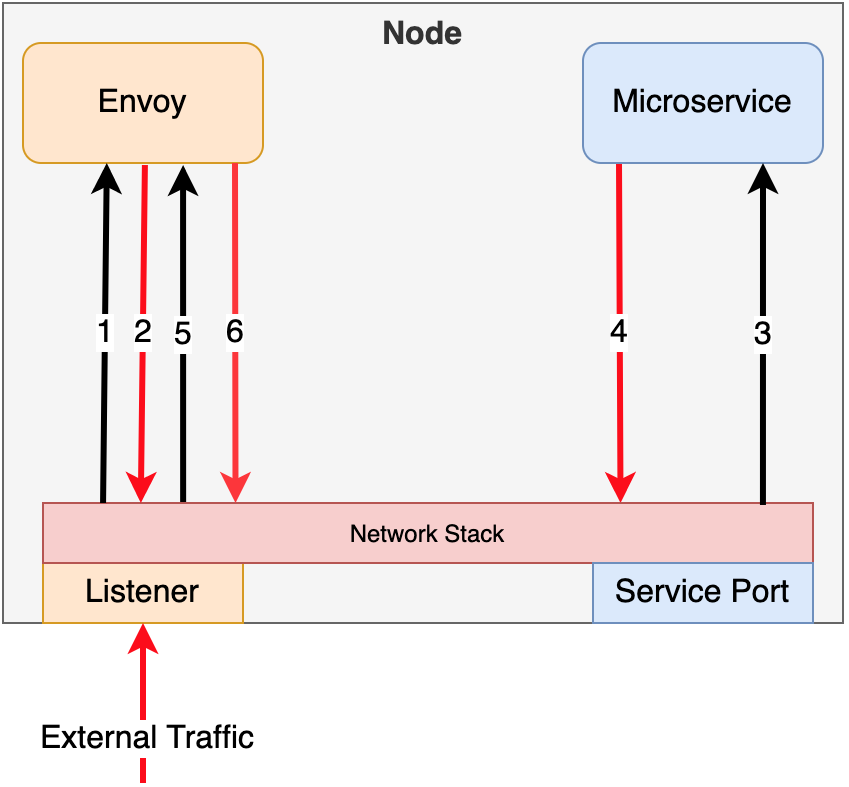
\includegraphics[keepaspectratio=true,width=3in]{figures/design/no_kmap.png}
        \caption{No Kmap Envoy Network Stack}
        \label{fig:no_kmap}
    \end{minipage}%
\end{figure}

\begin{figure}[!htb]
    \begin{minipage}{0.5\textwidth}
        \centering
        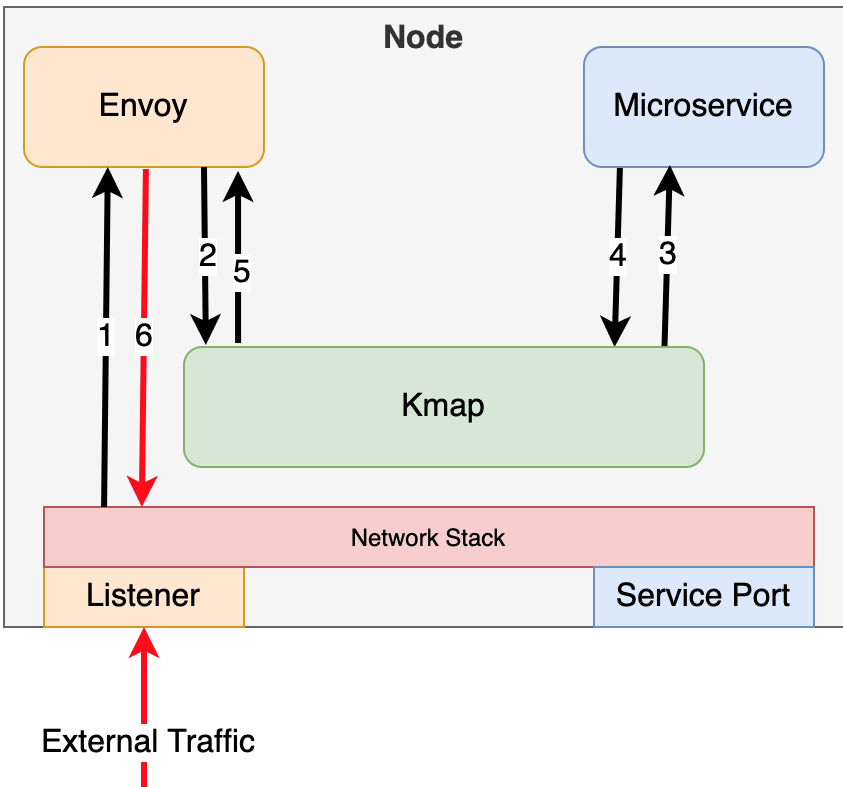
\includegraphics[keepaspectratio=true,width=3in]{figures/design/kmap.png}
        \caption{Kmap}
        \label{fig:kmap}
    \end{minipage}%
\end{figure}

\subsection{LD Preload}



\subsection{Pipe options}
Here, we outline potential methods for implementing the buffer \sysname uses to pass data between Envoy and the microservice.

\textbf{Named Pipes:}


\textbf{Unnamed Pipes:}


\textbf{Shared Memory:}


\subsection{When to apply \sysname}
The network stack has a very well defined, robust API which applications use to communicate.
A particular challenge for \sysname is pre-loading in front of those network calls and knowing when
to pass through the call, or when to route to the local buffer.
Since \sysname is designing primarily for Envoy, we use information about how it communicates with microservices to determine
which file descriptors should use \sysname.
This approach is not directly applicable to other sidecars (i.e. Linkerd) but is generalizable for applications, provided the applications work with Envoy first.


